Consider the sequence formed by starting from a positive integer $h_0$ and
iterating with $n = 1, 2, ...$ the following definition until $h_n = 1$:

\begin{center}
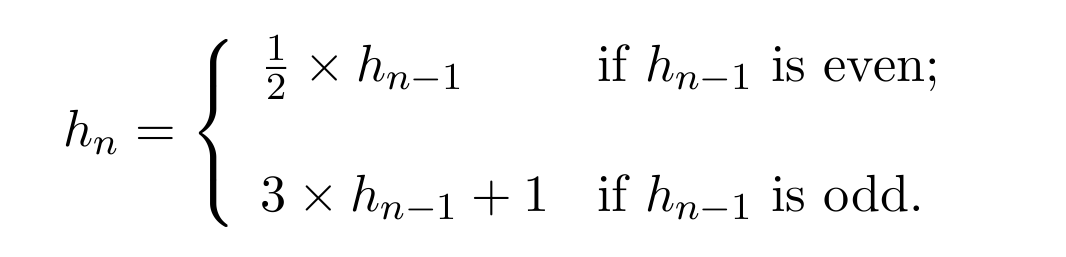
\includegraphics[scale=0.25]{problems/hailstone/imagens/hn.png}
\end{center}

For instance, if we start with $h_0 = 5$ the following sequence is generated: $5,
16, 8, 4, 2, 1$. If we
start with $h_0 = 11$, the sequence generated is $11, 34, 17, 52, 26, 13, 40,
20, 10, 5, 16, 8, 4, 2, 1.$
As you can see from these examples, the numbers go up and down, but
eventually comes down
to end in 1 (at least for all numbers that have ever been tried). These
sequences are called Hailstone
sequences because they are similar to the formation of hailstones, which get
carried upward by the
winds over and over again before they finally descend to the ground.
In this problem, given a positive integer, your task is to compute the
highest number in the
Hailstone sequence which starts with the given number.

\subsection*{Input}

Each test case is described using a single line. The line contains an integer
$H$ representing the starting value to build the sequence $(1 \leq H \leq 500)$.
The last test case is followed by a line containing one zero.

\subsection*{Output}

For each test case output a line with an integer representing the highest number
in the Hailstone sequence that starts with the given input value.

\begin{table}[!h]
\centering
\begin{tabular}{|l|l|}
\hline
\begin{minipage}[t]{3in}
\textbf{Sample Input}
\begin{verbatim}
5
11
27
0
\end{verbatim}
\vspace{1mm}
\end{minipage}
&

\begin{minipage}[t]{3in}
\textbf{Sample Output}
\begin{verbatim}
16
52
9232
\end{verbatim}
\vspace{1mm}
\end{minipage} \\
\hline
\end{tabular}
\end{table}

\newpage
